% Example of a section kept in its own file (latex/chapters/example.tex).
% It has no \documentclass or \begin{document}: it is only pasted into main.tex.
% First line of such files, so that Ctrl+Alt+B works from this tab too:
% !TEX root = ../../main.tex
\section{Results from the Python code}
    \label{s:results}
    % Numbers: write the macro defined in compute.py (here \ellA, \ellD, \Npeaks, \Hone).
    In the toy model the acoustic scale is $\ell_A=\ellA$ and the damping scale
    is $\ell_D=\ellD$. The spectrum has \Npeaks\ peaks below the multipole cut-off,
    and the first one has height $\Hone\,\mu\mathrm{K}^2$ (Table~\ref{tab:peaks}
    and Fig.~\ref{fig:spectrum}).

    % Table: latex/generated/table_peaks.tex is a bare tabular.
    \begin{table}[h]
        \centering
        \caption{First peaks of the toy spectrum (written by \texttt{compute.py}).}
        \label{tab:peaks}
        % AUTO-GENERATED by compute.py - do not edit by hand
\begin{tabular}{lcc}
\toprule
Peak & $\ell_{\rm peak}$ & Height [$\mu$K$^2$] \\
\midrule
$1$ & $298$ & $4.70\times10^{3}$ \\
$2$ & $596$ & $3.90\times10^{3}$ \\
$3$ & $894$ & $2.86\times10^{3}$ \\
$4$ & $1192$ & $1.85\times10^{3}$ \\
\bottomrule
\end{tabular}

    \end{table}

    % Plot: written by Python, exactly one column wide. \graphicspath (header.tex)
    % already points to latex/generated/ and latex/figures/, so the name is enough.
    % For a full-width plot use new_figure("full") in compute.py and a figure* here.
    \begin{figure}[t]
        \centering
        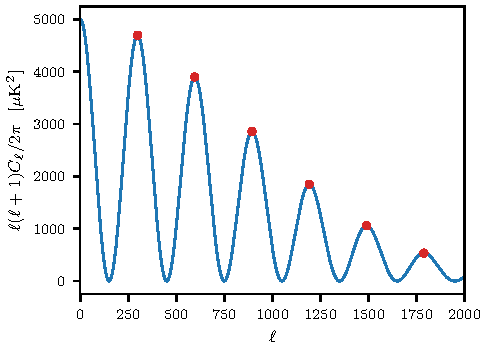
\includegraphics[width=\columnwidth]{fig_spectrum.pdf}
        \caption{Toy power spectrum (written by \texttt{compute.py}).}
        \label{fig:spectrum}
    \end{figure}

    